\documentclass{article}

\usepackage[utf8]{inputenc}
\usepackage{graphicx}		% Graphics.
\usepackage{color}
\usepackage[english]{babel}
\usepackage{float}
\usepackage{subcaption}
\usepackage{xfrac}
\usepackage{matlab-prettifier}
\usepackage{amsmath}    
\usepackage{amssymb}
\usepackage{siunitx}
\usepackage{pdfpages}
\usepackage{hyperref}
\usepackage{longtable}

% Create a separate table for the appendix.
\usepackage[toc,page]{appendix}

% Table of Content has fast links to sections.
\usepackage{hyperref}

% Remove dots in table of contents.
\usepackage[titles]{tocloft}
\renewcommand{\cftdot}{}

% Page style.
\usepackage[top=2cm, bottom=2cm, left = 2cm, right = 2cm]{geometry}
\setlength{\parindent}{0pt}	% Disable indents.

\begin{document}

%----------------------------------------------------------------------------------------
%	Title page.
%----------------------------------------------------------------------------------------
%----------------------------------------------------------------------------------------
%	TITLE PAGE.
%----------------------------------------------------------------------------------------

\begin{titlepage} % Suppresses displaying the page number on the title page and the subsequent page counts as page 1.
	\center % Centre everything on the page.
	\newcommand{\HRule}{\rule{\linewidth}{0.5mm}} % Defines a new command for horizontal lines, change thickness here.
	
	
	%------------------------------------------------
	%	Logo.
	%------------------------------------------------
	
\includegraphics[width=0.4\textwidth, trim=0 0 0 -2cm]{figures/LTU_logo.jpg}\\[1cm]
		
	
	%------------------------------------------------
	%	Headings.
	%------------------------------------------------
	\textsc{\Huge Lule\aa \ University of Technology}\\[1.5cm]
	
	\textsc{\LARGE Atmospheric Physics}\\[0.3cm]
	
	\textsc{\large F7004R}\\[0.5cm]
	
	
	%------------------------------------------------
	%	Title.
	%------------------------------------------------
	\HRule\\[0.4cm]
	
	{\Huge\bfseries Meteorological measurements radiosonde}\\[0.4cm]
	
	\HRule\\[1.5cm]
	
	
	%------------------------------------------------
	%	Author & supervisor.
	%------------------------------------------------
	\begin{minipage}{0.4\textwidth}
		\begin{flushleft}
			\large
			\textit{Authors}\\
			E.F.M. Weterings
			D. Talavera
		\end{flushleft}
	\end{minipage}
	~
	\begin{minipage}{0.4\textwidth}
		\begin{flushright}
			\large
			\textit{Supervisors}\\
			V. Barabash\\
			M. Milz
		\end{flushright}
	\end{minipage}
	
	
	%------------------------------------------------
	%	Date.
	%------------------------------------------------
	\vfill\vfill\vfill % Position the date 3/4 down the remaining page.
	
	{\large\today} % Date, change the \today to a set date if you want to be precise.
	
	
\end{titlepage}


%----------------------------------------------------------------------------------------
%	TABLE OF CONTENT.
%----------------------------------------------------------------------------------------
\newpage				% Start at new page.
\pagenumbering{arabic}	% Page numbering reset & style.
\renewcommand{\contentsname}{Table of Contents}
\tableofcontents		% Add table of content.


%----------------------------------------------------------------------------------------
%	QUESTION 1.
%----------------------------------------------------------------------------------------
\newpage
\section{Find Station No. 03808. Which location is this station attributed to? Where is it situated?}
As can be seen from figure \ref{fig:1}, the grounstation 03808 is located in south west part of England, more specifically in Camborne. 

\begin{figure}[H]
	\centering
 	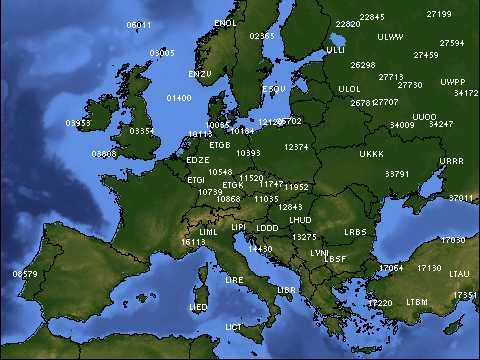
\includegraphics[width=1\textwidth]{figures/europe.jpg}
 	\caption{Europa weather stations \cite{assignment}.}
 	\label{fig:1}
\end{figure}


%----------------------------------------------------------------------------------------
%	QUESTION 2.
%----------------------------------------------------------------------------------------
\section{Extract the radiosonde profile data for 2007-07-05 0:00 UTC, 12:00 UTC and 2007-07-06 0:00 UTC}
% http://weather.uwyo.edu/cgi-bin/sounding?region=europe&TYPE=TEXT%3ALIST&YEAR=2007&MONTH=07&FROM=0500&TO=0600&STNM=03808
The information can be found online by clicking on the following URL:\\
\url{http://weather.uwyo.edu/cgi-bin/sounding?region=europe\&TYPE=TEXT%3ALIST&YEAR=2007&MONTH=07&FROM=0500&TO=0600&STNM=03808}\\

The information can also be found on the next page \cite{assignment}.
\newpage

\begin{longtable}{r|r|r|r|r|r|r|r|r|r|r}
\multicolumn{11}{c}{\textbf{03808 Camborne Observations at 00Z 05 Jul 2007}}\\ \hline

\multicolumn{1}{l}{PRES } & \multicolumn{1}{l}{HGHT } & \multicolumn{1}{l}{TEMP } & \multicolumn{1}{l}{DWPT } & \multicolumn{1}{l}{RELH} & \multicolumn{1}{l}{MIXR } & \multicolumn{1}{l}{DRCT } & \multicolumn{1}{l}{SKNT } & \multicolumn{1}{l}{THAT} & \multicolumn{1}{l}{ THTE} & \multicolumn{1}{l}{THTV} \\
\multicolumn{1}{l}{[hPa]} & \multicolumn{1}{l}{[m]} & \multicolumn{1}{l}{[C]} & \multicolumn{1}{l}{[C] } & \multicolumn{1}{l}{[\%]} & \multicolumn{1}{l}{[g/kg]} & \multicolumn{1}{l}{[deg]} & \multicolumn{1}{l}{[knot]} & \multicolumn{1}{l}{[K]} & \multicolumn{1}{l}{[K]} & \multicolumn{1}{l}{[K]} \\ \hline
1007 & 88 & 13.6 & 11.1 & 85 & 8.3 & 290 & 15 & 286.2 & 309.5 & 287.6 \\
1005 & 104 & 13.6 & 11.2 & 85 & 8.37 & 290 & 17 & 286.3 & 309.8 & 287.8 \\
1000 & 143 & 13.4 & 11.1 & 86 & 8.36 & 290 & 20 & 286.6 & 310 & 288 \\
994 & 194 & 12.9 & 10.8 & 87 & 8.25 & 290 & 25 & 286.6 & 309.8 & 288 \\
985 & 270 & 12.2 & 10.4 & 89 & 8.1 & 290 & 26 & 286.6 & 309.4 & 288 \\
956 & 520 & 9.9 & 9.2 & 96 & 7.72 & 290 & 31 & 286.7 & 308.4 & 288 \\
950 & 572 & 9.4 & 9 & 97 & 7.64 & 290 & 31 & 286.7 & 308.3 & 288 \\
937 & 686 & 8.4 & 8.4 & 100 & 7.43 & 290 & 32 & 286.8 & 307.8 & 288.1 \\
925 & 793 & 7.8 & 7.8 & 100 & 7.22 & 290 & 32 & 287.3 & 307.7 & 288.5 \\
895 & 1066 & 6.2 & 6.2 & 100 & 6.68 & 302 & 28 & 288.4 & 307.4 & 289.5 \\
888 & 1130 & 6 & 6 & 100 & 6.66 & 305 & 27 & 288.8 & 307.9 & 290 \\
878 & 1224 & 5.8 & 5.8 & 100 & 6.63 & 304 & 28 & 289.5 & 308.5 & 290.7 \\
853 & 1461 & 4.4 & 4.4 & 100 & 6.18 & 300 & 29 & 290.4 & 308.3 & 291.5 \\
850 & 1490 & 4.4 & 4.2 & 99 & 6.12 & 300 & 29 & 290.7 & 308.5 & 291.8 \\
847 & 1519 & 4.2 & 3.6 & 96 & 5.88 & 300 & 29 & 290.8 & 307.9 & 291.9 \\
828 & 1704 & 4.6 & -0.4 & 70 & 4.51 & 300 & 32 & 293.1 & 306.5 & 293.9 \\
825 & 1733 & 4.6 & -0.6 & 69 & 4.46 & 300 & 32 & 293.4 & 306.7 & 294.2 \\
814 & 1842 & 4.6 & -1.4 & 65 & 4.26 & 300 & 32 & 294.6 & 307.3 & 295.3 \\
786 & 2127 & 2.6 & -1.7 & 73 & 4.32 & 300 & 34 & 295.4 & 308.4 & 296.2 \\
779 & 2199 & 2.4 & -2.4 & 71 & 4.13 & 300 & 34 & 295.9 & 308.4 & 296.7 \\
772 & 2272 & 3.2 & -4.8 & 56 & 3.48 & 300 & 34 & 297.6 & 308.2 & 298.2 \\
761 & 2388 & 3 & -6.7 & 49 & 3.05 & 300 & 35 & 298.5 & 308 & 299.1 \\
746 & 2549 & 2.6 & -9.4 & 41 & 2.53 & 299 & 35 & 299.8 & 307.8 & 300.3 \\
705 & 3003 & -0.3 & -12.3 & 40 & 2.12 & 295 & 37 & 301.5 & 308.3 & 301.9 \\
700 & 3060 & -0.7 & -12.7 & 40 & 2.07 & 295 & 37 & 301.7 & 308.3 & 302.1 \\
674 & 3360 & -2.7 & -16.3 & 34 & 1.6 & 295 & 36 & 302.8 & 308 & 303.1 \\
653 & 3611 & -4.3 & -19.3 & 30 & 1.28 & 295 & 38 & 303.7 & 307.9 & 303.9 \\
633 & 3856 & -5.3 & -36.3 & 7 & 0.27 & 295 & 41 & 305.2 & 306.2 & 305.3 \\
631 & 3880 & -5.5 & -36.5 & 7 & 0.27 & 295 & 41 & 305.3 & 306.3 & 305.4 \\
585 & 4469 & -9.5 & -42.5 & 5 & 0.16 & 295 & 44 & 307.3 & 307.9 & 307.3 \\
576 & 4589 & -10.4 & -43.5 & 5 & 0.14 & 295 & 45 & 307.6 & 308.1 & 307.6 \\
568 & 4696 & -11.3 & -44.3 & 5 & 0.13 & 295 & 48 & 307.8 & 308.3 & 307.8 \\
552 & 4915 & -11.6 & -41.4 & 6 & 0.18 & 295 & 53 & 309.9 & 310.6 & 310 \\
534 & 5169 & -12 & -38 & 9 & 0.27 & 305 & 63 & 312.4 & 313.4 & 312.5 \\
529 & 5241 & -12.1 & -37.1 & 11 & 0.3 & 303 & 66 & 313.1 & 314.3 & 313.2 \\
520 & 5372 & -12.7 & -27.7 & 27 & 0.76 & 301 & 71 & 313.9 & 316.7 & 314.1 \\
518 & 5401 & -12.9 & -27.1 & 29 & 0.8 & 300 & 72 & 314 & 316.9 & 314.2 \\
507 & 5565 & -14.1 & -24.1 & 43 & 1.08 & 300 & 68 & 314.5 & 318.3 & 314.7 \\
500 & 5670 & -14.7 & -25.7 & 39 & 0.95 & 300 & 66 & 315.1 & 318.4 & 315.2 \\
495 & 5746 & -15.1 & -27.1 & 35 & 0.84 & 300 & 65 & 315.5 & 318.5 & 315.6 \\
493 & 5776 & -15.4 & -26.7 & 38 & 0.88 & 300 & 64 & 315.5 & 318.6 & 315.6 \\
472 & 6103 & -18.7 & -22 & 75 & 1.4 & 303 & 65 & 315.3 & 320.2 & 315.6 \\
458 & 6327 & -20 & -24.1 & 70 & 1.19 & 305 & 65 & 316.4 & 320.6 & 316.6 \\
455 & 6376 & -20.3 & -24.6 & 68 & 1.15 & 305 & 66 & 316.6 & 320.7 & 316.9 \\
438 & 6657 & -21.9 & -39.9 & 18 & 0.27 & 305 & 73 & 318.1 & 319.1 & 318.1 \\
416 & 7035 & -24.5 & -42.5 & 17 & 0.22 & 305 & 82 & 319.5 & 320.3 & 319.5 \\
409 & 7158 & -24.8 & -49.1 & 9 & 0.11 & 305 & 85 & 320.7 & 321.1 & 320.7 \\
405 & 7230 & -24.9 & -52.9 & 6 & 0.07 & 303 & 85 & 321.4 & 321.7 & 321.4 \\
400 & 7320 & -25.3 & -58.3 & 3 & 0.04 & 300 & 85 & 322 & 322.2 & 322 \\
398 & 7356 & -25.5 & -57 & 4 & 0.04 & 300 & 85 & 322.2 & 322.4 & 322.2 \\
396 & 7393 & -25.7 & -55.7 & 4 & 0.05 & 301 & 85 & 322.4 & 322.6 & 322.4 \\
383 & 7635 & -27.3 & -44.3 & 18 & 0.2 & 306 & 86 & 323.4 & 324.2 & 323.4 \\
373 & 7824 & -28.7 & -43.4 & 23 & 0.22 & 310 & 86 & 324 & 324.9 & 324 \\
350 & 8279 & -32.1 & -41.1 & 40 & 0.3 & 306 & 91 & 325.4 & 326.6 & 325.4 \\
345 & 8380 & -33 & -40.9 & 45 & 0.31 & 305 & 92 & 325.5 & 326.8 & 325.6 \\
326 & 8776 & -36.4 & -40 & 69 & 0.36 & 305 & 100 & 326.2 & 327.6 & 326.2 \\
322 & 8863 & -37.1 & -39.8 & 76 & 0.37 & 306 & 101 & 326.3 & 327.8 & 326.4 \\
316 & 8993 & -37.7 & -40.7 & 73 & 0.35 & 307 & 103 & 327.2 & 328.6 & 327.3 \\
302 & 9305 & -40.1 & -47.1 & 47 & 0.18 & 310 & 107 & 328.1 & 328.9 & 328.1 \\
300 & 9350 & -40.5 & -47.5 & 47 & 0.18 & 310 & 108 & 328.2 & 328.9 & 328.2 \\
298 & 9395 & -40.8 & -47.3 & 49 & 0.18 & 310 & 108 & 328.4 & 329.1 & 328.4 \\
292 & 9534 & -41.7 & -46.7 & 58 & 0.2 & 310 & 109 & 329 & 329.8 & 329.1 \\
282 & 9769 & -42.9 & -50.9 & 41 & 0.13 & 310 & 110 & 330.6 & 331.1 & 330.6 \\
271 & 10035 & -45.2 & -51.3 & 50 & 0.13 & 310 & 112 & 331 & 331.5 & 331 \\
265 & 10185 & -46.5 & -51.5 & 57 & 0.13 & 313 & 119 & 331.2 & 331.8 & 331.3 \\
260 & 10311 & -46.8 & -55.2 & 38 & 0.08 & 315 & 125 & 332.6 & 332.9 & 332.6 \\
259 & 10337 & -46.9 & -55.9 & 35 & 0.08 & 315 & 125 & 332.8 & 333.1 & 332.8 \\
250 & 10570 & -48.9 & -59.9 & 27 & 0.05 & 310 & 122 & 333.2 & 333.4 & 333.2 \\
248 & 10623 & -49.1 & -59.1 & 30 & 0.05 & 310 & 122 & 333.7 & 333.9 & 333.7 \\
235 & 10972 & -51.1 & -62.6 & 24 & 0.04 & 310 & 120 & 335.9 & 336.1 & 335.9 \\
231 & 11084 & -51.7 & -63.7 & 22 & 0.03 & 310 & 118 & 336.6 & 336.7 & 336.6 \\
217 & 11486 & -53.5 & -67.5 & 17 & 0.02 & 310 & 109 & 339.9 & 340 & 339.9 \\
206 & 11820 & -52.9 & -70 & 11 & 0.01 & 310 & 103 & 346 & 346 & 346 \\
201 & 11978 & -52.6 & -71.3 & 9 & 0.01 & 305 & 90 & 348.9 & 348.9 & 348.9 \\
200 & 12010 & -52.5 & -71.5 & 8 & 0.01 & 305 & 89 & 349.5 & 349.5 & 349.5 \\
190 & 12341 & -51.9 & -73.9 & 5 & 0.01 & 299 & 86 & 355.6 & 355.6 & 355.6 \\
183 & 12584 & -51.3 & -77 & 3 & 0.01 & 295 & 83 & 360.4 & 360.5 & 360.4 \\
179 & 12727 & -50.9 & -78.9 & 2 & 0 & 298 & 78 & 363.3 & 363.4 & 363.3 \\
177 & 12800 & -51.3 & -79.7 & 2 & 0 & 300 & 76 & 363.9 & 363.9 & 363.9 \\
170 & 13061 & -52.7 & -82.5 & 2 & 0 & 295 & 69 & 365.8 & 365.8 & 365.8 \\
169 & 13099 & -52.9 & -82.9 & 1 & 0 & 295 & 70 & 366 & 366.1 & 366 \\
162 & 13372 & -51.8 & -82.9 & 1 & 0 & 295 & 77 & 372.4 & 372.4 & 372.4 \\
157 & 13575 & -50.9 & -82.9 & 1 & 0 & 304 & 68 & 377.2 & 377.2 & 377.2 \\
154 & 13700 & -51.6 & -84 & 1 & 0 & 310 & 63 & 378.1 & 378.1 & 378.1 \\
150 & 13870 & -52.5 & -85.5 & 1 & 0 & 305 & 61 & 379.4 & 379.4 & 379.4 \\
149 & 13913 & -52.7 & -85.7 & 1 & 0 & 303 & 61 & 379.8 & 379.8 & 379.8 \\
145 & 14090 & -52.3 & -85.3 & 1 & 0 & 295 & 63 & 383.5 & 383.5 & 383.5 \\
142 & 14226 & -52 & -85 & 1 & 0 & 305 & 64 & 386.3 & 386.3 & 386.3 \\
135 & 14554 & -51.2 & -84.2 & 1 & 0 & 305 & 52 & 393.3 & 393.3 & 393.3 \\
134 & 14602 & -51.1 & -84.1 & 1 & 0 & 305 & 52 & 394.3 & 394.3 & 394.3 \\
124 & 15106 & -51.7 & -84.7 & 1 & 0 & 300 & 49 & 402.1 & 402.1 & 402.1 \\
114 & 15652 & -52.3 & -85.3 & 1 & 0 & 310 & 41 & 410.7 & 410.7 & 410.7 \\
105 & 16185 & -52.5 & -85.5 & 1 & 0 & 310 & 36 & 420.1 & 420.1 & 420.1 \\
100 & 16500 & -53.3 & -86.3 & 1 & 0 & 310 & 33 & 424.5 & 424.5 & 424.5 \\
93 & 16966 & -54.3 & -86.8 & 1 & 0 & 300 & 27 & 431.3 & 431.3 & 431.3 \\
88.2 & 17306 & -55.1 & -87.1 & 1 & 0 & 294 & 23 & 436.4 & 436.4 & 436.4 \\
85 & 17543 & -55 & -87 & 1 & 0 & 290 & 20 & 441.2 & 441.2 & 441.2 \\
80 & 17931 & -54.8 & -86.8 & 1 & 0 & 305 & 17 & 449.3 & 449.3 & 449.3 \\
76.6 & 18209 & -54.7 & -86.7 & 1 & 0 & 311 & 17 & 455.1 & 455.2 & 455.1 \\
74 & 18432 & -53.7 & -86.1 & 1 & 0 & 315 & 17 & 461.8 & 461.8 & 461.8 \\
71 & 18698 & -52.5 & -85.4 & 1 & 0 & 10 & 8 & 469.9 & 469.9 & 469.9 \\
70.6 & 18735 & -52.3 & -85.3 & 1 & 0 & 6 & 8 & 471 & 471 & 471 \\
70 & 18790 & -52.7 & -85.7 & 1 & 0 & 0 & 8 & 471.3 & 471.3 & 471.3 \\
67.4 & 19033 & -54.5 & -87.5 & 1 & 0 & 315 & 8 & 472.5 & 472.5 & 472.5 \\
66 & 19167 & -53.6 & -86.7 & 1 & 0 & 290 & 8 & 477.2 & 477.2 & 477.2 \\
63.2 & 19445 & -51.9 & -84.9 & 1 & 0 & 327 & 10 & 487 & 487 & 487 \\
63 & 19466 & -51.9 & -84.9 & 1 & 0 & 330 & 10 & 487.5 & 487.5 & 487.5 \\
61 & 19674 & -51.8 & -84.8 & 1 & 0 & 40 & 7 & 492.2 & 492.2 & 492.2 \\
57 & 20113 & -51.6 & -84.6 & 1 & 0.01 & 295 & 7 & 502.2 & 502.3 & 502.2 \\
55 & 20344 & -51.5 & -84.5 & 1 & 0.01 & 0 & 0 & 507.6 & 507.6 & 507.6 \\
54.5 & 20403 & -51.5 & -84.5 & 1 & 0.01 & 347 & 1 & 509 & 509 & 509 \\
52 & 20706 & -51.5 & -84.5 & 1 & 0.01 & 280 & 6 & 515.9 & 515.9 & 515.9 \\
50 & 20960 & -51.5 & -84.5 & 1 & 0.01 & 5 & 5 & 521.7 & 521.7 & 521.7 \\
49.3 & 21052 & -51.1 & -85.1 & 1 & 0.01 & 360 & 5 & 524.7 & 524.8 & 524.7 \\
48 & 21226 & -50.1 & -84.1 & 1 & 0.01 & 350 & 6 & 531.2 & 531.3 & 531.2 \\
47.8 & 21253 & -49.9 & -83.9 & 1 & 0.01 & 358 & 7 & 532.2 & 532.3 & 532.2 \\
47 & 21364 & -49.9 & -83.9 & 1 & 0.01 & 30 & 10 & 534.7 & 534.8 & 534.7 \\
46 & 21504 & -50 & -84 & 1 & 0.01 & 90 & 11 & 537.9 & 537.9 & 537.9 \\
44 & 21795 & -50.1 & -84.1 & 1 & 0.01 & 135 & 6 & 544.5 & 544.6 & 544.5 \\
43.9 & 21810 & -50.1 & -84.1 & 1 & 0.01 & 128 & 6 & 544.8 & 544.9 & 544.8 \\
43.1 & 21931 & -49.3 & -83.3 & 1 & 0.01 & 71 & 5 & 549.7 & 549.8 & 549.7 \\
42 & 22100 & -49.3 & -83.3 & 1 & 0.01 & 350 & 3 & 553.8 & 553.9 & 553.8 \\
40 & 22421 & -49.2 & -83.2 & 1 & 0.01 & 175 & 3 & 561.8 & 561.8 & 561.8 \\
38 & 22757 & -49.1 & -83.2 & 1 & 0.01 & 90 & 4 & 570.2 & 570.3 & 570.2 \\
36.4 & 23040 & -49.1 & -83.1 & 1 & 0.01 & 67 & 7 & 577.4 & 577.5 & 577.4 \\
34 & 23488 & -49.1 & -83.1 & 1 & 0.01 & 30 & 12 & 588.7 & 588.9 & 588.7 \\
30 & 24310 & -49.1 & -83.1 & 1 & 0.01 & 70 & 7 & 610.2 & 610.3 & 610.2 \\
29.4 & 24443 & -49.1 & -83.1 & 1 & 0.01 & 63 & 8 & 613.7 & 613.8 & 613.7 \\
28 & 24763 & -48.8 & -82.8 & 1 & 0.02 & 45 & 9 & 623.1 & 623.2 & 623.1 \\
27.4 & 24905 & -48.7 & -82.7 & 1 & 0.02 & 60 & 13 & 627.3 & 627.5 & 627.3 \\
27 & 25001 & -48.9 & -82.9 & 1 & 0.02 & 70 & 16 & 629.3 & 629.5 & 629.3 \\
26.7 & 25075 & -49.1 & -83.1 & 1 & 0.02 & 71 & 16 & 630.8 & 631 & 630.8 \\
24.3 & 25695 & -47.5 & -82.5 & 1 & 0.02 & 79 & 17 & 652.7 & 652.9 & 652.7 \\
24 &   &   &   &   &   & 80 & 17 &   &   &  \\
\end{longtable}%

\begin{longtable}{l|r}
\multicolumn{2}{c}{\textbf{Station information and sounding indices}} \\ \hline
Station number & 3808 \\
Observation time & \multicolumn{1}{l}{ 070705/0000} \\
Station latitude & 50.22 \\
Station longitude & -5.32 \\
Station elevation & 88 \\
Showalter index & 8.64 \\
Lifted index & 8.22 \\
LIFT computed using virtual temperature & 8.18 \\
SWEAT index & 174.41 \\
K index & 11.3 \\
Cross totals index & 18.9 \\
Vertical totals index & 19.1 \\
Totals totals index & 38 \\
Convective Available Potential Energy & 14.21 \\
CAPE using virtual temperature & 15.51 \\
Convective Inhibition & 0 \\
CINS using virtual temperature & 0 \\
Equilibrum Level & 844.14 \\
Equilibrum Level using virtual temperature & 842.9 \\
Level of Free Convection & 953.06 \\
LFCT using virtual temperature & 954.64 \\
Bulk Richardson Number & 0.64 \\
Bulk Richardson Number using CAPV & 0.7 \\
Temp [K] of the Lifted Condensation Level & 282.93 \\
Pres [hPa] of the Lifted Condensation Level & 956.04 \\
Mean mixed layer potential temperature & 286.6 \\
Mean mixed layer mixing ratio & 8.01 \\
1000 hPa to 500 hPa thickness & 5527 \\
Precipitable water [mm] for entire sounding & 19.63 \\
\end{longtable}%


\newpage

% Table generated by Excel2LaTeX from sheet 'Sheet2'
\begin{longtable}{r|r|r|r|r|r|r|r|r|r|r}
\multicolumn{11}{c}{\textbf{03808 Camborne Observations at 12Z 05 Jul 2007}}\\ \hline
\multicolumn{1}{l}{PRES } & \multicolumn{1}{l}{HGHT } & \multicolumn{1}{l}{TEMP } & \multicolumn{1}{l}{DWPT } & \multicolumn{1}{l}{RELH } & \multicolumn{1}{l}{MIXR } & \multicolumn{1}{l}{DRCT } & \multicolumn{1}{l}{SKNT } & \multicolumn{1}{l}{THAT } & \multicolumn{1}{l}{ THTE } & \multicolumn{1}{l}{THTV } \\
\multicolumn{1}{l}{[hPa]} & \multicolumn{1}{l}{[m]} & \multicolumn{1}{l}{[C]} & \multicolumn{1}{l}{[C] } & \multicolumn{1}{l}{[\%]} & \multicolumn{1}{l}{[g/kg]} & \multicolumn{1}{l}{[deg]} & \multicolumn{1}{l}{[knot]} & \multicolumn{1}{l}{[K]} & \multicolumn{1}{l}{[K]} & \multicolumn{1}{l}{[K]} \\ \hline
1002 & 88 & 13.6 & 13.4 & 99 & 9.73 & 180 & 15 & 286.6 & 313.8 & 288.3 \\
1001 & 99 & 13.4 & 13.3 & 99 & 9.67 & 180 & 16 & 286.5 & 313.5 & 288.1 \\
1000 & 109 & 13.2 & 13 & 99 & 9.49 & 180 & 17 & 286.4 & 312.9 & 288 \\
998 & 126 & 13 & 13 & 100 & 9.51 & 180 & 19 & 286.3 & 312.9 & 287.9 \\
994 & 160 & 12.8 & 12.8 & 100 & 9.43 & 180 & 24 & 286.5 & 312.8 & 288.1 \\
989 & 202 & 12.6 & 12.6 & 100 & 9.34 & 175 & 25 & 286.6 & 312.8 & 288.2 \\
985 & 236 & 12.4 & 12.4 & 100 & 9.26 & 180 & 27 & 286.8 & 312.7 & 288.4 \\
972 & 347 & 12 & 12 & 100 & 9.14 & 195 & 32 & 287.5 & 313.2 & 289.1 \\
963 & 425 & 11.7 & 11.7 & 100 & 9.05 & 195 & 35 & 287.9 & 313.5 & 289.5 \\
952 & 521 & 11.4 & 11.4 & 100 & 8.95 & 205 & 36 & 288.6 & 313.8 & 290.1 \\
943 & 601 & 11.1 & 11.1 & 100 & 8.86 & 205 & 36 & 289 & 314.1 & 290.6 \\
928 & 735 & 10.6 & 10.6 & 100 & 8.72 & 213 & 35 & 289.9 & 314.7 & 291.4 \\
925 & 762 & 10.6 & 10.6 & 100 & 8.75 & 215 & 35 & 290.1 & 315.1 & 291.7 \\
923 & 780 & 10.6 & 10.6 & 100 & 8.74 & 220 & 35 & 290.3 & 315.2 & 291.8 \\
900 & 991 & 10.2 & 10.1 & 99 & 8.69 & 238 & 36 & 292 & 317 & 293.5 \\
886 & 1122 & 10.8 & 10.8 & 100 & 9.26 & 248 & 37 & 293.9 & 320.7 & 295.6 \\
866 & 1313 & 10.4 & 10 & 97 & 8.98 & 264 & 38 & 295.4 & 321.6 & 297.1 \\
865 & 1323 & 10.4 & 10.1 & 97 & 9.02 & 265 & 38 & 295.6 & 321.9 & 297.2 \\
859 & 1381 & 10.7 & 10.4 & 98 & 9.29 & 270 & 43 & 296.4 & 323.5 & 298.1 \\
855 & 1420 & 10.8 & 10.6 & 99 & 9.47 & 268 & 45 & 296.9 & 324.6 & 298.6 \\
852 & 1449 & 11.4 & 11.3 & 99 & 9.96 & 266 & 46 & 297.9 & 327.1 & 299.7 \\
850 & 1469 & 11.4 & 11.1 & 98 & 9.85 & 265 & 47 & 298.1 & 327 & 299.8 \\
842 & 1548 & 11.2 & 10.1 & 93 & 9.3 & 266 & 46 & 298.7 & 326.1 & 300.3 \\
810 & 1871 & 9.2 & 7.1 & 87 & 7.87 & 269 & 44 & 299.9 & 323.3 & 301.3 \\
804 & 1933 & 8.8 & 6.9 & 88 & 7.81 & 270 & 43 & 300.1 & 323.4 & 301.5 \\
773 & 2258 & 6.6 & 5.7 & 94 & 7.48 & 267 & 46 & 301.1 & 323.6 & 302.5 \\
744 & 2571 & 5 & 4.3 & 95 & 7.03 & 265 & 48 & 302.6 & 323.9 & 303.9 \\
727 & 2760 & 4 & 3.4 & 96 & 6.76 & 270 & 45 & 303.6 & 324.2 & 304.8 \\
713 & 2918 & 3 & 1.4 & 89 & 5.99 & 275 & 43 & 304.2 & 322.6 & 305.3 \\
710 & 2952 & 2.8 & 1 & 88 & 5.83 & 275 & 43 & 304.3 & 322.2 & 305.4 \\
700 & 3067 & 2 & 0.7 & 91 & 5.78 & 275 & 42 & 304.7 & 322.5 & 305.7 \\
676 & 3348 & 0.2 & -1 & 92 & 5.29 & 273 & 42 & 305.7 & 322.1 & 306.7 \\
648 & 3686 & -1.3 & -3.5 & 85 & 4.59 & 270 & 41 & 307.8 & 322.2 & 308.6 \\
640 & 3785 & -1.7 & -4.2 & 83 & 4.4 & 271 & 41 & 308.4 & 322.3 & 309.2 \\
607 & 4205 & -3.9 & -9.9 & 63 & 2.98 & 277 & 42 & 310.5 & 320.2 & 311.1 \\
601 & 4284 & -3.9 & -18.9 & 30 & 1.44 & 278 & 43 & 311.4 & 316.3 & 311.7 \\
594 & 4376 & -4.3 & -19.3 & 30 & 1.41 & 280 & 43 & 312 & 316.8 & 312.3 \\
593 & 4389 & -4.4 & -19.3 & 30 & 1.4 & 280 & 43 & 312 & 316.8 & 312.3 \\
582 & 4535 & -5.8 & -19.6 & 33 & 1.39 & 270 & 45 & 312 & 316.8 & 312.3 \\
565 & 4767 & -8.1 & -20.1 & 37 & 1.38 & 280 & 50 & 312 & 316.7 & 312.3 \\
557 & 4878 & -8.7 & -13.2 & 70 & 2.5 & 280 & 46 & 312.6 & 320.9 & 313.1 \\
551 & 4962 & -8.3 & -11.2 & 80 & 2.97 & 280 & 43 & 314 & 323.8 & 314.6 \\
537 & 5161 & -9.3 & -12.2 & 79 & 2.8 & 280 & 35 & 315.1 & 324.4 & 315.7 \\
529 & 5277 & -9.9 & -12.8 & 79 & 2.7 & 275 & 32 & 315.8 & 324.8 & 316.3 \\
518 & 5439 & -10.7 & -13.7 & 79 & 2.58 & 277 & 37 & 316.7 & 325.4 & 317.2 \\
511 & 5543 & -11.7 & -14.3 & 81 & 2.49 & 278 & 41 & 316.7 & 325.1 & 317.2 \\
500 & 5710 & -12.3 & -15.8 & 75 & 2.24 & 280 & 46 & 318 & 325.6 & 318.4 \\
495 & 5787 & -12.7 & -16.4 & 74 & 2.16 & 280 & 50 & 318.4 & 325.8 & 318.9 \\
479 & 6037 & -13.9 & -18.3 & 69 & 1.9 & 280 & 55 & 319.9 & 326.5 & 320.3 \\
455 & 6423 & -16.9 & -20.7 & 72 & 1.63 & 280 & 62 & 320.9 & 326.6 & 321.2 \\
426 & 6917 & -20.7 & -23.7 & 77 & 1.33 & 285 & 52 & 322.1 & 326.9 & 322.4 \\
424 & 6951 & -20.9 & -23.9 & 77 & 1.31 & 285 & 51 & 322.3 & 327 & 322.6 \\
400 & 7380 & -23.5 & -26.8 & 74 & 1.07 & 290 & 61 & 324.4 & 328.3 & 324.6 \\
397 & 7435 & -23.8 & -27.2 & 74 & 1.04 & 290 & 60 & 324.6 & 328.4 & 324.8 \\
389 & 7583 & -24.8 & -28.3 & 72 & 0.96 & 280 & 64 & 325.3 & 328.8 & 325.5 \\
376 & 7831 & -26.3 & -30.1 & 70 & 0.84 & 285 & 71 & 326.4 & 329.6 & 326.6 \\
375 & 7850 & -26.5 & -30.2 & 71 & 0.83 & 285 & 72 & 326.5 & 329.6 & 326.6 \\
358 & 8185 & -29.3 & -31.7 & 80 & 0.76 & 287 & 72 & 327 & 329.9 & 327.2 \\
340 & 8553 & -31.3 & -36.3 & 61 & 0.51 & 290 & 73 & 329.2 & 331.1 & 329.3 \\
339 & 8573 & -31.4 & -36.4 & 61 & 0.5 & 290 & 73 & 329.2 & 331.2 & 329.3 \\
316 & 9069 & -34.9 & -39.9 & 60 & 0.38 & 290 & 82 & 331.1 & 332.6 & 331.2 \\
304 & 9338 & -36.9 & -40.3 & 71 & 0.38 & 290 & 87 & 332 & 333.5 & 332.1 \\
300 & 9430 & -37.3 & -41.9 & 62 & 0.32 & 290 & 89 & 332.7 & 334 & 332.8 \\
294 & 9569 & -38.4 & -43.8 & 57 & 0.27 & 295 & 91 & 333.1 & 334.2 & 333.1 \\
290 & 9663 & -39.1 & -45.1 & 53 & 0.24 & 293 & 91 & 333.4 & 334.3 & 333.4 \\
284 & 9803 & -40.3 & -46.3 & 53 & 0.21 & 290 & 92 & 333.7 & 334.6 & 333.7 \\
261 & 10371 & -44.9 & -50.9 & 51 & 0.14 & 290 & 97 & 335 & 335.6 & 335 \\
256 & 10501 & -46 & -52 & 51 & 0.12 & 285 & 98 & 335.3 & 335.8 & 335.3 \\
251 & 10633 & -47.1 & -53.1 & 50 & 0.11 & 285 & 106 & 335.6 & 336 & 335.6 \\
250 & 10660 & -47.3 & -53.3 & 50 & 0.11 & 285 & 106 & 335.6 & 336.1 & 335.6 \\
249 & 10686 & -47.3 & -53.3 & 50 & 0.11 & 285 & 106 & 336 & 336.5 & 336 \\
235 & 11060 & -50.8 & -57.1 & 47 & 0.07 & 290 & 106 & 336.3 & 336.6 & 336.3 \\
231 & 11171 & -51.8 & -58.3 & 46 & 0.06 & 285 & 107 & 336.4 & 336.7 & 336.4 \\
228 & 11255 & -52.6 & -59.2 & 45 & 0.06 & 285 & 111 & 336.5 & 336.7 & 336.5 \\
213 & 11695 & -56.7 & -63.7 & 41 & 0.03 & 285 & 104 & 336.7 & 336.9 & 336.7 \\
209 & 11814 & -57.5 & -63.9 & 44 & 0.03 & 285 & 102 & 337.3 & 337.5 & 337.3 \\
202 & 12028 & -58.9 & -64.2 & 50 & 0.03 & 290 & 99 & 338.4 & 338.5 & 338.4 \\
200 & 12090 & -59.3 & -64.3 & 52 & 0.03 & 290 & 97 & 338.7 & 338.9 & 338.7 \\
195 & 12250 & -58.1 & -66.9 & 31 & 0.02 & 290 & 89 & 343.1 & 343.2 & 343.1 \\
191 & 12381 & -57.1 & -69.1 & 20 & 0.02 & 286 & 93 & 346.7 & 346.8 & 346.7 \\
190 & 12415 & -57 & -69.5 & 19 & 0.02 & 285 & 94 & 347.3 & 347.4 & 347.3 \\
184 & 12619 & -56.8 & -71.6 & 14 & 0.01 & 290 & 103 & 351 & 351.1 & 351 \\
180 & 12759 & -56.5 & -73.1 & 11 & 0.01 & 295 & 100 & 353.5 & 353.6 & 353.5 \\
179 & 12794 & -56.5 & -73.5 & 10 & 0.01 & 296 & 96 & 354.2 & 354.2 & 354.2 \\
175 & 12939 & -54.4 & -74.6 & 7 & 0.01 & 300 & 80 & 359.9 & 359.9 & 359.9 \\
174 & 12976 & -53.9 & -74.9 & 6 & 0.01 & 300 & 79 & 361.4 & 361.4 & 361.4 \\
170 & 13127 & -53 & -77.2 & 4 & 0.01 & 300 & 77 & 365.3 & 365.3 & 365.3 \\
163 & 13400 & -51.3 & -81.3 & 2 & 0 & 307 & 59 & 372.5 & 372.5 & 372.5 \\
160 & 13520 & -51.7 & -82.4 & 1 & 0 & 310 & 51 & 373.8 & 373.8 & 373.8 \\
154 & 13769 & -52.5 & -84.6 & 1 & 0 & 295 & 43 & 376.5 & 376.5 & 376.5 \\
150 & 13940 & -53.1 & -86.1 & 1 & 0 & 295 & 47 & 378.4 & 378.4 & 378.4 \\
144 & 14202 & -53.5 & -85.5 & 1 & 0 & 295 & 50 & 382.1 & 382.1 & 382.1 \\
138 & 14474 & -53.6 & -85.8 & 1 & 0 & 295 & 53 & 386.6 & 386.6 & 386.6 \\
135 & 14615 & -53.7 & -86 & 1 & 0 & 300 & 58 & 388.9 & 388.9 & 388.9 \\
131 & 14808 & -53.8 & -86.3 & 1 & 0 & 300 & 51 & 392.1 & 392.1 & 392.1 \\
127 & 15006 & -53.9 & -86.5 & 1 & 0 & 295 & 46 & 395.4 & 395.4 & 395.4 \\
125 & 15108 & -53.9 & -86.6 & 1 & 0 & 290 & 47 & 397.1 & 397.1 & 397.1 \\
121 & 15316 & -54 & -86.9 & 1 & 0 & 310 & 45 & 400.6 & 400.6 & 400.6 \\
119 & 15423 & -54.1 & -87 & 1 & 0 & 315 & 41 & 402.5 & 402.5 & 402.5 \\
118 & 15477 & -54.1 & -87.1 & 1 & 0 & 311 & 39 & 403.4 & 403.4 & 403.4 \\
115 & 15641 & -54.7 & -87.3 & 1 & 0 & 300 & 33 & 405.3 & 405.3 & 405.3 \\
113 & 15752 & -55.1 & -87.4 & 1 & 0 & 295 & 35 & 406.6 & 406.6 & 406.6 \\
111 & 15866 & -55.5 & -87.5 & 1 & 0 & 296 & 36 & 407.9 & 407.9 & 407.9 \\
106 & 16159 & -55.2 & -87.2 & 1 & 0 & 300 & 39 & 413.8 & 413.8 & 413.8 \\
100 & 16530 & -54.9 & -86.9 & 1 & 0 & 310 & 31 & 421.4 & 421.4 & 421.4 \\
85 & 17567 & -56.9 & -88.9 & 1 & 0 & 320 & 22 & 437.4 & 437.5 & 437.4 \\
83.3 & 17696 & -57.1 & -89.1 & 1 & 0 & 319 & 21 & 439.5 & 439.5 & 439.5 \\
77 & 18199 & -55.4 & -87.9 & 1 & 0 & 315 & 17 & 453 & 453 & 453 \\
70.5 & 18764 & -53.5 & -86.5 & 1 & 0 & 329 & 9 & 468.6 & 468.6 & 468.6 \\
70 & 18810 & -53.5 & -86.5 & 1 & 0 & 330 & 8 & 469.6 & 469.6 & 469.6 \\
66 & 19186 & -55.2 & -87.4 & 1 & 0 & 5 & 3 & 473.8 & 473.8 & 473.8 \\
65.4 & 19244 & -55.5 & -87.5 & 1 & 0 & 344 & 4 & 474.4 & 474.4 & 474.4 \\
64 & 19382 & -54.3 & -86.8 & 1 & 0 & 295 & 7 & 479.9 & 480 & 479.9 \\
62.1 & 19575 & -52.7 & -85.7 & 1 & 0 & 322 & 6 & 487.7 & 487.7 & 487.7 \\
56 & 20240 & -52.7 & -85.7 & 1 & 0 & 55 & 3 & 502.3 & 502.3 & 502.3 \\
53.1 & 20583 & -52.7 & -85.7 & 1 & 0 & 171 & 10 & 510 & 510 & 510 \\
53 & 20595 & -52.7 & -85.7 & 1 & 0 & 175 & 10 & 510.3 & 510.3 & 510.3 \\
51 & 20842 & -52.4 & -85.4 & 1 & 0.01 & 300 & 7 & 516.5 & 516.6 & 516.5 \\
50 & 20970 & -52.3 & -85.3 & 1 & 0.01 & 340 & 4 & 519.8 & 519.8 & 519.8 \\
49 & 21101 & -52.1 & -85.2 & 1 & 0.01 & 65 & 2 & 523.2 & 523.3 & 523.2 \\
41 & 22260 & -50.4 & -84.3 & 1 & 0.01 & 95 & 6 & 554.9 & 554.9 & 554.9 \\
39.8 & 22453 & -50.1 & -84.1 & 1 & 0.01 & 94 & 7 & 560.3 & 560.4 & 560.3 \\
36.5 & 23021 & -48.3 & -82.3 & 1 & 0.01 & 91 & 10 & 579 & 579.1 & 579 \\
36 & 23111 & -48.7 & -82.7 & 1 & 0.01 & 90 & 11 & 580.4 & 580.5 & 580.4 \\
35 & 23296 & -49.4 & -83.4 & 1 & 0.01 & 110 & 8 & 583.1 & 583.2 & 583.2 \\
34.3 & 23429 & -49.9 & -83.9 & 1 & 0.01 & 89 & 8 & 585.2 & 585.3 & 585.2 \\
33 & 23682 & -48.7 & -82.7 & 1 & 0.01 & 50 & 8 & 594.7 & 594.9 & 594.7 \\
32.3 & 23823 & -48.1 & -82.1 & 1 & 0.01 & 71 & 17 & 600.1 & 600.2 & 600.1 \\
32 & 23885 & -48.1 & -82.1 & 1 & 0.01 & 80 & 21 & 601.7 & 601.8 & 601.7 \\
30 & 24310 & -48.1 & -82.1 & 1 & 0.02 & 100 & 13 & 612.9 & 613 & 612.9 \\
29 & 24534 & -48.1 & -82.1 & 1 & 0.02 & 85 & 11 & 618.9 & 619 & 618.9 \\
27 & 25006 & -48.1 & -82.1 & 1 & 0.02 & 65 & 12 & 631.6 & 631.8 & 631.6 \\
26 & 25255 & -48.1 & -82.1 & 1 & 0.02 & 70 & 23 & 638.5 & 638.6 & 638.5 \\
25 & 25514 & -48.1 & -82.1 & 1 & 0.02 & 110 & 15 & 645.7 & 645.9 & 645.7 \\
24 & 25785 & -46.7 & -81.2 & 1 & 0.02 & 115 & 9 & 657.4 & 657.6 & 657.4 \\
23.2 & 26011 & -45.5 & -80.5 & 1 & 0.03 & 79 & 10 & 667.2 & 667.5 & 667.2 \\
23 & 26068 & -45.6 & -80.6 & 1 & 0.03 & 70 & 10 & 668.7 & 668.9 & 668.7 \\
21 & 26675 & -46.3 & -81.3 & 1 & 0.03 & 80 & 21 & 684.1 & 684.3 & 684.1 \\
20.5 & 26836 & -46.5 & -81.5 & 1 & 0.03 & 80 & 21 & 688.2 & 688.5 & 688.2 \\
20 & 27000 & -46.1 & -81.1 & 1 & 0.03 & 80 & 21 & 694.3 & 694.6 & 694.3 \\
19 & 27343 & -45.4 & -80.6 & 1 & 0.03 & 95 & 16 & 706.8 & 707.1 & 706.8 \\
17 & 28087 & -43.8 & -79.5 & 1 & 0.04 & 80 & 17 & 734.6 & 735.1 & 734.6 \\
15.7 & 28619 & -42.7 & -78.7 & 1 & 0.05 & 86 & 27 & 755.1 & 755.7 & 755.2 \\
15 & 28929 & -42.2 & -78.4 & 1 & 0.06 & 90 & 32 & 766.7 & 767.3 & 766.7 \\
13 & 29899 & -40.7 & -77.4 & 1 & 0.08 & 90 & 22 & 804 & 804.9 & 804 \\
12.1 & 30386 & -39.9 & -76.9 & 1 & 0.09 & 99 & 26 & 823.4 & 824.5 & 823.4 \\
12 & 30443 & -39.7 & -76.8 & 1 & 0.09 & 100 & 26 & 826.1 & 827.2 & 826.1 \\
10 & 31700 & -34.9 & -73.9 & 1 & 0.17 & 80 & 15 & 888.1 & 890.3 & 888.2 \\
9.6 & 31985 & -34.1 & -73.1 & 1 & 0.2 & 80 & 20 & 901.5 & 904.2 & 901.6 \\
9 & 32439 & -32.4 & -72 & 1 & 0.25 & 80 & 29 & 924.9 & 928.2 & 925 \\
8.7 & 32678 & -31.5 & -71.5 & 1 & 0.28 &   &   & 937.3 & 941.1 & 937.5 \\
8 & 33272 & -31.3 & -71.3 & 1 & 0.32 &   &   & 960.9 & 965.2 & 961 \\
\end{longtable}%

\newpage
\begin{longtable}{l|r}
\multicolumn{2}{c}{\textbf{Station information and sounding indices}
}\\ \hline
Station number & 3808 \\
Observation time & \multicolumn{1}{l}{ 070705/1200} \\
Station latitude & 50.22 \\
Station longitude & -5.32 \\
Station elevation & 88 \\
Showalter index & 0.49 \\
Lifted index & 8.07 \\
LIFT computed using virtual temperature & 8.19 \\
SWEAT index & 273.22 \\
K index & 33.5 \\
Cross totals index & 23.4 \\
Vertical totals index & 23.7 \\
Totals totals index & 47.1 \\
Convective Available Potential Energy & 0 \\
CAPE using virtual temperature & 0 \\
Convective Inhibition & 0 \\
CINS using virtual temperature & 0 \\
Equilibrum Level & 969.83 \\
Equilibrum Level using virtual temperature & 969.84 \\
Level of Free Convection & 973.09 \\
LFCT using virtual temperature & 973.09 \\
Bulk Richardson Number & 0 \\
Bulk Richardson Number using CAPV & 0 \\
Temp [K] of the Lifted Condensation Level & 285.22 \\
Pres [hPa] of the Lifted Condensation Level & 973.09 \\
Mean mixed layer potential temperature & 287.47 \\
Mean mixed layer mixing ratio & 9.18 \\
1000 hPa to 500 hPa thickness & 5601 \\
Precipitable water [mm] for entire sounding & 34.7 \\
\end{longtable}%

\newpage

% Table generated by Excel2LaTeX from sheet 'Sheet3'
\begin{longtable}{|r|r|r|r|r|r|r|r|r|r|r}
\multicolumn{11}{c}{\textbf{03808 Camborne Observations at 00Z 06 Jul 2007}} \\ \hline
\multicolumn{1}{l}{PRES } & \multicolumn{1}{l}{HGHT } & \multicolumn{1}{l}{TEMP } & \multicolumn{1}{l}{DWPT } & \multicolumn{1}{l}{RELH } & \multicolumn{1}{l}{MIXR } & \multicolumn{1}{l}{DRCT } & \multicolumn{1}{l}{SKNT } & \multicolumn{1}{l}{THAT } & \multicolumn{1}{l}{ THTE } & \multicolumn{1}{l}{THTV } \\
\multicolumn{1}{l}{[hPa]} & \multicolumn{1}{l}{[m]} & \multicolumn{1}{l}{[C]} & \multicolumn{1}{l}{[C] } & \multicolumn{1}{l}{[\%]} & \multicolumn{1}{l}{[g/kg]} & \multicolumn{1}{l}{[deg]} & \multicolumn{1}{l}{[knot]} & \multicolumn{1}{l}{[K]} & \multicolumn{1}{l}{[K]} & \multicolumn{1}{l}{[K]} \\ \hline
1003 & 88 & 13.4 & 10 & 80 & 7.74 & 280 & 16 & 286.3 & 308.1 & 287.6 \\
1001 & 103 & 13.6 & 10.3 & 80 & 7.91 & 279 & 17 & 286.7 & 309 & 288 \\
1000 & 111 & 13.4 & 10.1 & 80 & 7.81 & 279 & 18 & 286.6 & 308.6 & 287.9 \\
988 & 212 & 12.7 & 9.6 & 82 & 7.64 & 275 & 26 & 286.8 & 308.4 & 288.1 \\
965 & 410 & 11.2 & 8.6 & 84 & 7.31 & 281 & 33 & 287.3 & 308 & 288.5 \\
948 & 557 & 9.7 & 7.8 & 88 & 7.06 & 285 & 38 & 287.2 & 307.2 & 288.4 \\
932 & 699 & 8.2 & 7.1 & 93 & 6.83 & 285 & 37 & 287.1 & 306.4 & 288.2 \\
925 & 761 & 7.8 & 7 & 95 & 6.84 & 285 & 37 & 287.3 & 306.7 & 288.5 \\
916 & 842 & 7 & 6.5 & 96 & 6.65 & 285 & 39 & 287.3 & 306.2 & 288.4 \\
897 & 1014 & 5.4 & 5.3 & 99 & 6.26 & 293 & 36 & 287.3 & 305.2 & 288.4 \\
891 & 1069 & 5.5 & 4.7 & 94 & 6.04 & 295 & 35 & 288 & 305.3 & 289.1 \\
887 & 1106 & 5.6 & 4.3 & 91 & 5.9 & 296 & 36 & 288.5 & 305.4 & 289.5 \\
875 & 1218 & 5 & 2.9 & 86 & 5.42 & 300 & 40 & 289 & 304.6 & 289.9 \\
872 & 1246 & 5.6 & 2.8 & 82 & 5.4 & 299 & 40 & 289.9 & 305.5 & 290.8 \\
862 & 1340 & 5.2 & 1.5 & 77 & 4.97 & 295 & 42 & 290.4 & 304.9 & 291.3 \\
852 & 1436 & 5.2 & -0.8 & 65 & 4.25 & 291 & 43 & 291.4 & 304 & 292.1 \\
850 & 1455 & 5.6 & -1.4 & 61 & 4.08 & 290 & 43 & 292 & 304.1 & 292.7 \\
838 & 1572 & 6.3 & -5.3 & 43 & 3.08 & 285 & 45 & 293.9 & 303.3 & 294.5 \\
827 & 1680 & 7 & -9 & 31 & 2.35 & 288 & 46 & 295.8 & 303.1 & 296.2 \\
820 & 1750 & 6.9 & -10.2 & 28 & 2.16 & 290 & 47 & 296.4 & 303.1 & 296.8 \\
814 & 1810 & 6.8 & -11.2 & 26 & 2.01 & 286 & 49 & 296.9 & 303.2 & 297.3 \\
810 & 1850 & 7.4 & -17.6 & 15 & 1.19 & 283 & 51 & 298 & 301.9 & 298.2 \\
806 & 1891 & 7.2 & -17.5 & 15 & 1.21 & 280 & 52 & 298.2 & 302.2 & 298.4 \\
794 & 2014 & 6.8 & -17.2 & 16 & 1.26 & 280 & 50 & 299 & 303.1 & 299.2 \\
774 & 2224 & 7 & -31 & 5 & 0.37 & 280 & 48 & 301.4 & 302.8 & 301.5 \\
768 & 2287 & 6.7 & -30.6 & 5 & 0.39 & 280 & 47 & 301.8 & 303.2 & 301.9 \\
756 & 2416 & 6.2 & -29.8 & 5 & 0.43 & 279 & 48 & 302.6 & 304.1 & 302.7 \\
727 & 2735 & 3.9 & -32.1 & 5 & 0.36 & 275 & 50 & 303.5 & 304.8 & 303.5 \\
716 & 2859 & 3 & -33 & 5 & 0.33 & 273 & 50 & 303.8 & 305 & 303.9 \\
700 & 3041 & 2 & -36 & 4 & 0.25 & 270 & 50 & 304.7 & 305.6 & 304.7 \\
697 & 3076 & 2 & -36 & 4 & 0.26 & 270 & 50 & 305 & 306 & 305.1 \\
688 & 3180 & 1.2 & -37.1 & 4 & 0.23 & 270 & 51 & 305.4 & 306.2 & 305.4 \\
670 & 3392 & -0.3 & -39.4 & 3 & 0.19 & 275 & 50 & 306 & 306.7 & 306 \\
649 & 3647 & -2.1 & -42.1 & 3 & 0.15 & 274 & 55 & 306.7 & 307.2 & 306.7 \\
600 & 4267 & -4.5 & -44.5 & 3 & 0.12 & 270 & 67 & 310.8 & 311.3 & 310.9 \\
593 & 4359 & -4.9 & -44.9 & 3 & 0.12 & 270 & 66 & 311.4 & 311.9 & 311.5 \\
584 & 4479 & -5.6 & -45.9 & 3 & 0.11 & 270 & 64 & 312 & 312.4 & 312 \\
562 & 4779 & -7.3 & -48.3 & 2 & 0.09 & 270 & 65 & 313.4 & 313.8 & 313.4 \\
544 & 5032 & -9.3 & -47 & 3 & 0.1 & 270 & 66 & 314 & 314.4 & 314.1 \\
540 & 5089 & -9.7 & -46.7 & 3 & 0.11 & 267 & 65 & 314.2 & 314.6 & 314.2 \\
538 & 5118 & -9.8 & -46.9 & 3 & 0.1 & 265 & 65 & 314.3 & 314.8 & 314.4 \\
517 & 5424 & -11.3 & -49.3 & 3 & 0.08 & 268 & 72 & 316.2 & 316.5 & 316.2 \\
510 & 5528 & -11.3 & -39.3 & 8 & 0.25 & 269 & 74 & 317.4 & 318.4 & 317.4 \\
500 & 5680 & -12.5 & -31.5 & 19 & 0.55 & 270 & 77 & 317.7 & 319.8 & 317.8 \\
481 & 5974 & -14.2 & -28 & 30 & 0.8 & 270 & 84 & 319.2 & 322.1 & 319.4 \\
464 & 6246 & -15.7 & -24.7 & 46 & 1.12 & 268 & 87 & 320.6 & 324.6 & 320.8 \\
456 & 6377 & -15.9 & -30.9 & 26 & 0.64 & 267 & 88 & 321.9 & 324.3 & 322.1 \\
450 & 6477 & -16.3 & -27.3 & 38 & 0.91 & 266 & 89 & 322.7 & 326 & 322.9 \\
443 & 6593 & -17.2 & -27.6 & 40 & 0.9 & 265 & 90 & 322.9 & 326.2 & 323.1 \\
429 & 6832 & -19.2 & -28.1 & 45 & 0.89 & 265 & 85 & 323.4 & 326.7 & 323.6 \\
410 & 7169 & -21.9 & -28.9 & 53 & 0.86 & 274 & 91 & 324.1 & 327.3 & 324.3 \\
409 & 7187 & -22 & -28.7 & 55 & 0.88 & 275 & 91 & 324.2 & 327.4 & 324.4 \\
400 & 7350 & -23.1 & -26.8 & 72 & 1.07 & 270 & 94 & 324.9 & 328.8 & 325.1 \\
399 & 7368 & -23.3 & -26.8 & 73 & 1.08 & 270 & 94 & 324.9 & 328.8 & 325.1 \\
385 & 7628 & -25.1 & -27.9 & 77 & 1 & 270 & 95 & 325.9 & 329.6 & 326.1 \\
372 & 7878 & -26.8 & -29 & 81 & 0.94 & 270 & 103 & 326.8 & 330.3 & 327 \\
371 & 7897 & -26.9 & -29.1 & 82 & 0.93 & 271 & 103 & 326.9 & 330.4 & 327.1 \\
363 & 8053 & -28.4 & -30 & 86 & 0.88 & 275 & 100 & 326.9 & 330.2 & 327.1 \\
349 & 8335 & -31.1 & -31.7 & 94 & 0.78 & 275 & 102 & 327 & 329.9 & 327.1 \\
345 & 8416 & -31.3 & -31.7 & 96 & 0.79 & 275 & 102 & 327.8 & 330.7 & 327.9 \\
339 & 8541 & -31.5 & -35.1 & 70 & 0.57 & 275 & 103 & 329.2 & 331.4 & 329.3 \\
331 & 8710 & -31.7 & -39.7 & 45 & 0.37 & 275 & 106 & 331.1 & 332.6 & 331.2 \\
320 & 8949 & -32.5 & -46.5 & 23 & 0.18 & 275 & 110 & 333.2 & 334 & 333.3 \\
313 & 9104 & -33.7 & -48.7 & 21 & 0.15 & 275 & 113 & 333.7 & 334.3 & 333.7 \\
300 & 9400 & -36.3 & -50.3 & 22 & 0.13 & 270 & 111 & 334.1 & 334.6 & 334.1 \\
297 & 9470 & -36.9 & -50.7 & 23 & 0.12 & 270 & 108 & 334.2 & 334.7 & 334.2 \\
286 & 9731 & -39.1 & -52.1 & 24 & 0.11 & 268 & 111 & 334.7 & 335.1 & 334.7 \\
273 & 10047 & -41.9 & -53.5 & 27 & 0.1 & 265 & 115 & 335.1 & 335.5 & 335.1 \\
265 & 10249 & -43.7 & -54.3 & 30 & 0.09 & 270 & 108 & 335.3 & 335.7 & 335.3 \\
260 & 10378 & -44.9 & -54.9 & 32 & 0.09 & 268 & 107 & 335.4 & 335.8 & 335.4 \\
250 & 10640 & -47.3 & -55.3 & 39 & 0.08 & 265 & 105 & 335.6 & 336 & 335.6 \\
249 & 10666 & -47.5 & -55.3 & 40 & 0.08 & 265 & 106 & 335.6 & 336 & 335.7 \\
236 & 11015 & -50.6 & -55.9 & 54 & 0.08 & 270 & 105 & 336.1 & 336.5 & 336.1 \\
231 & 11155 & -51.9 & -56.1 & 60 & 0.08 & 274 & 97 & 336.3 & 336.6 & 336.3 \\
229 & 11211 & -51.7 & -56.8 & 54 & 0.08 & 275 & 94 & 337.4 & 337.8 & 337.4 \\
223 & 11382 & -51.1 & -59.1 & 38 & 0.06 & 270 & 96 & 340.9 & 341.2 & 340.9 \\
207 & 11860 & -53.8 & -63.9 & 28 & 0.03 & 265 & 105 & 344 & 344.1 & 344 \\
200 & 12080 & -55.1 & -66.1 & 24 & 0.03 & 270 & 112 & 345.4 & 345.5 & 345.4 \\
193 & 12307 & -56.5 & -68.5 & 21 & 0.02 & 270 & 114 & 346.6 & 346.7 & 346.6 \\
192 & 12341 & -56 & -68.8 & 19 & 0.02 & 275 & 115 & 348 & 348.1 & 348 \\
184 & 12615 & -51.7 & -71.2 & 8 & 0.01 & 280 & 92 & 359.1 & 359.2 & 359.1 \\
181 & 12721 & -50.1 & -72.1 & 6 & 0.01 & 282 & 82 & 363.5 & 363.6 & 363.5 \\
178 & 12831 & -50 & -74.1 & 4 & 0.01 & 285 & 71 & 365.4 & 365.5 & 365.4 \\
171 & 13093 & -49.7 & -79 & 2 & 0 & 275 & 60 & 370 & 370.1 & 370 \\
170 & 13132 & -49.7 & -79.7 & 2 & 0 & 274 & 61 & 370.7 & 370.8 & 370.7 \\
163 & 13407 & -50.2 & -81 & 1 & 0 & 265 & 67 & 374.4 & 374.4 & 374.4 \\
159 & 13569 & -50.5 & -81.7 & 1 & 0 & 270 & 71 & 376.6 & 376.6 & 376.6 \\
153 & 13821 & -50.9 & -82.9 & 1 & 0 & 275 & 69 & 380 & 380 & 380 \\
150 & 13950 & -50.1 & -84.1 & 1 & 0 & 275 & 59 & 383.5 & 383.6 & 383.5 \\
148 & 14038 & -49.4 & -83.4 & 1 & 0 & 275 & 54 & 386.2 & 386.2 & 386.2 \\
147 & 14082 & -49.1 & -83.1 & 1 & 0 & 275 & 55 & 387.5 & 387.5 & 387.5 \\
142 & 14308 & -50.6 & -84.6 & 1 & 0 & 275 & 60 & 388.7 & 388.7 & 388.7 \\
141 & 14354 & -50.9 & -84.9 & 1 & 0 & 277 & 59 & 389 & 389 & 389 \\
136 & 14588 & -51.4 & -85.2 & 1 & 0 & 285 & 52 & 392.1 & 392.1 & 392.1 \\
125 & 15134 & -52.5 & -85.8 & 1 & 0 & 285 & 35 & 399.6 & 399.6 & 399.6 \\
123 & 15238 & -52.8 & -85.9 & 1 & 0 & 275 & 31 & 401.1 & 401.1 & 401.1 \\
120 & 15398 & -53.1 & -86.1 & 1 & 0 & 268 & 33 & 403.3 & 403.3 & 403.3 \\
119 & 15451 & -53.3 & -86.2 & 1 & 0 & 265 & 34 & 403.9 & 403.9 & 403.9 \\
113 & 15781 & -54.6 & -87.2 & 1 & 0 & 270 & 42 & 407.5 & 407.5 & 407.5 \\
106 & 16189 & -56.1 & -88.4 & 1 & 0 & 290 & 31 & 412 & 412.1 & 412 \\
103 & 16373 & -56.9 & -88.9 & 1 & 0 & 275 & 33 & 414.1 & 414.1 & 414.1 \\
102 & 16435 & -57.1 & -89.1 & 1 & 0 & 275 & 34 & 414.8 & 414.8 & 414.8 \\
100 & 16560 & -56.9 & -88.9 & 1 & 0 & 280 & 36 & 417.5 & 417.5 & 417.5 \\
96 & 16819 & -56.7 & -88.7 & 1 & 0 & 280 & 36 & 422.8 & 422.8 & 422.8 \\
91.7 & 17111 & -56.5 & -88.5 & 1 & 0 & 277 & 29 & 428.8 & 428.8 & 428.8 \\
89 & 17302 & -55 & -87.5 & 1 & 0 & 275 & 25 & 435.4 & 435.4 & 435.4 \\
86.7 & 17469 & -53.7 & -86.7 & 1 & 0 & 289 & 21 & 441.3 & 441.3 & 441.3 \\
85 & 17596 & -54.4 & -87.1 & 1 & 0 & 300 & 18 & 442.5 & 442.5 & 442.5 \\
80 & 17981 & -56.5 & -88.4 & 1 & 0 & 305 & 9 & 445.9 & 445.9 & 445.9 \\
74.5 & 18435 & -58.9 & -89.9 & 1 & 0 & 293 & 14 & 449.9 & 450 & 449.9 \\
73.4 & 18529 & -56.7 & -88.7 & 1 & 0 & 291 & 15 & 456.5 & 456.5 & 456.5 \\
73 & 18564 & -56.8 & -88.8 & 1 & 0 & 290 & 15 & 457 & 457 & 457 \\
71.7 & 18678 & -57.1 & -89.1 & 1 & 0 & 292 & 15 & 458.7 & 458.7 & 458.7 \\
70 & 18830 & -56.7 & -88.7 & 1 & 0 & 295 & 16 & 462.7 & 462.8 & 462.7 \\
67.7 & 19044 & -53.7 & -86.7 & 1 & 0 & 333 & 14 & 473.6 & 473.7 & 473.6 \\
67 & 19110 & -54 & -86.8 & 1 & 0 & 345 & 14 & 474.4 & 474.4 & 474.4 \\
66 & 19206 & -54.5 & -87 & 1 & 0 & 0 & 10 & 475.5 & 475.5 & 475.5 \\
63.7 & 19434 & -55.5 & -87.5 & 1 & 0 & 340 & 5 & 478 & 478 & 478 \\
62 & 19607 & -54.8 & -87.1 & 1 & 0 & 325 & 1 & 483.2 & 483.3 & 483.2 \\
59 & 19925 & -53.6 & -86.4 & 1 & 0 & 315 & 6 & 492.9 & 493 & 492.9 \\
58.4 & 19991 & -53.3 & -86.3 & 1 & 0 & 351 & 4 & 495 & 495 & 495 \\
58 & 20035 & -53.5 & -86.5 & 1 & 0 & 15 & 3 & 495.4 & 495.4 & 495.4 \\
56.5 & 20204 & -54.5 & -87.5 & 1 & 0 & 38 & 4 & 496.9 & 497 & 496.9 \\
53 & 20615 & -53.7 & -86.7 & 1 & 0 & 95 & 7 & 508 & 508.1 & 508.1 \\
51 & 20863 & -53.2 & -86.2 & 1 & 0 & 280 & 3 & 514.8 & 514.9 & 514.8 \\
50 & 20990 & -52.9 & -85.9 & 1 & 0 & 300 & 3 & 518.4 & 518.4 & 518.4 \\
49 & 21120 & -52.6 & -85.6 & 1 & 0.01 & 70 & 4 & 522.1 & 522.1 & 522.1 \\
48.7 & 21160 & -52.5 & -85.5 & 1 & 0.01 & 64 & 4 & 523.2 & 523.3 & 523.2 \\
46.2 & 21500 & -52.9 & -85.9 & 1 & 0.01 & 9 & 2 & 530.2 & 530.2 & 530.2 \\
46 & 21529 & -52.8 & -85.8 & 1 & 0.01 & 5 & 2 & 531.1 & 531.1 & 531.1 \\
45 & 21671 & -52.3 & -85.5 & 1 & 0.01 & 55 & 10 & 535.6 & 535.6 & 535.6 \\
44 & 21817 & -51.9 & -85.2 & 1 & 0.01 & 90 & 10 & 540.2 & 540.2 & 540.2 \\
43 & 21966 & -51.4 & -84.9 & 1 & 0.01 & 70 & 5 & 545 & 545 & 545 \\
42 & 22119 & -50.9 & -84.6 & 1 & 0.01 & 40 & 10 & 549.9 & 549.9 & 549.9 \\
40.5 & 22355 & -50.1 & -84.1 & 1 & 0.01 & 44 & 14 & 557.5 & 557.6 & 557.5 \\
40 & 22436 & -50.4 & -84.3 & 1 & 0.01 & 45 & 16 & 558.7 & 558.8 & 558.7 \\
38 & 22770 & -51.8 & -84.9 & 1 & 0.01 & 105 & 15 & 563.6 & 563.6 & 563.6 \\
37.5 & 22856 & -52.1 & -85.1 & 1 & 0.01 & 107 & 15 & 564.8 & 564.9 & 564.8 \\
35 & 23305 & -50.9 & -84.3 & 1 & 0.01 & 120 & 14 & 579.3 & 579.4 & 579.3 \\
34 & 23494 & -50.4 & -84 & 1 & 0.01 & 140 & 10 & 585.4 & 585.5 & 585.4 \\
33 & 23688 & -49.8 & -83.7 & 1 & 0.01 & 0 & 0 & 591.9 & 592 & 591.9 \\
32.4 & 23808 & -49.5 & -83.5 & 1 & 0.01 & 13 & 3 & 595.8 & 595.9 & 595.8 \\
31 & 24096 & -50.6 & -84.6 & 1 & 0.01 & 45 & 10 & 600.4 & 600.5 & 600.4 \\
30.4 & 24224 & -51.1 & -85.1 & 1 & 0.01 & 69 & 14 & 602.4 & 602.5 & 602.5 \\
30 & 24310 & -50.9 & -84.9 & 1 & 0.01 & 85 & 16 & 605.3 & 605.4 & 605.3 \\
29 & 24531 & -49.6 & -83.6 & 1 & 0.01 & 75 & 20 & 614.8 & 614.9 & 614.8 \\
28.8 & 24577 & -49.3 & -83.3 & 1 & 0.01 &   &   & 616.8 & 616.9 & 616.8 \\
27 & 24999 & -49.5 & -83.5 & 1 & 0.01 &   &   & 627.7 & 627.8 & 627.7 \\
\end{longtable}%

\newpage
% Table generated by Excel2LaTeX from sheet 'Sheet3'
\begin{longtable}{l|r}
\multicolumn{2}{c}{\textbf{Station information and sounding indices}} \\ \hline
Station number & 3808 \\
Observation time & \multicolumn{1}{l}{ 070706/0000} \\
Station latitude & 50.22 \\
Station longitude & -5.32 \\
Station elevation & 88 \\
Showalter index & 13.67 \\
Lifted index & 11.14 \\
LIFT computed using virtual temperature & 11.05 \\
SWEAT index & 163.01 \\
K index & -21.3 \\
Cross totals index & 11.1 \\
Vertical totals index & 18.1 \\
Totals totals index & 29.2 \\
Convective Available Potential Energy & 9.48 \\
CAPE using virtual temperature & 11.65 \\
Convective Inhibition & -0.34 \\
CINS using virtual temperature & -0.1 \\
Equilibrum Level & 873.37 \\
Equilibrum Level using virtual temperature & 872.72 \\
Level of Free Convection & 932.58 \\
LFCT using virtual temperature & 934.66 \\
Bulk Richardson Number & 0.16 \\
Bulk Richardson Number using CAPV & 0.19 \\
Temp [K] of the Lifted Condensation Level & 281.52 \\
Pres [hPa] of the Lifted Condensation Level & 934.95 \\
Mean mixed layer potential temperature & 286.99 \\
Mean mixed layer mixing ratio & 7.44 \\
1000 hPa to 500 hPa thickness & 5569 \\
Precipitable water [mm] for entire sounding & 13.92 \\
\end{longtable}%




%----------------------------------------------------------------------------------------
%	QUESTION 3.
%----------------------------------------------------------------------------------------
\newpage
\section{Plot the profiles of temperature T, dewpoint temperature $T_D$ and relative humidity RH for each of theses dates. (T and $T_D$ in one plot, RH in a separate one) Use a suitable altitude coordinate!}



%----------------------------------------------------------------------------------------
%	QUESTION 4.
%----------------------------------------------------------------------------------------
\newpage
\section{How are T and $T_D$ related to each other? Consider RH for your argumentation}
The dew point temperature ($T_D$) is the temperature of which the air must be cooled to to become saturated with water vapour. This is dependent on the current temperature and the relative humidity (RH). When the temperature increases, it can hold more water vapour and thus the dew point temperature increases for the same relative humidity (RH). When the relative humidity increases, under the same temperature, then the dew point temperature goes up as well. The correlation between these parameters can be seen in figure \ref{fig:Q4}.\\

\begin{figure}[H]
	\centering
	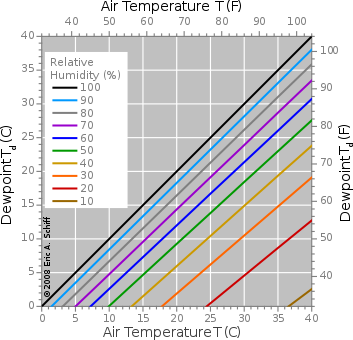
\includegraphics[width=.5\textwidth]{figures/Dewpoint-RH.png}
	\caption{Air temperature, dewpoint and relative humidity relation \cite{wikiQ4}.}
	\label{fig:Q4}
\end{figure}

When cooled below the dew point temperature, the airborne water vapor will condense to form liquid water (dew). When air cools to its dew point through contact with a surface that is colder than the air, water will condense on the surface.\\

The dew point temperature can be calculated using equation \ref{eq:4-1} \cite{wikiQ4}.
\begin{equation}
T_D = \frac{c \gamma (T, RH)}{b - \gamma (T, RH)} \label{eq:4-1}
\end{equation}

With $\gamma (T, RH)$ being given by equation \ref{eq:4-2} \cite{wikiQ4}.
\begin{equation}
\gamma (T, RH) = ln \left( \frac{RH}{100} \right) + \frac{bT}{c + T} \label{eq:4-2}
\end{equation}

The constants $b$ and $c$ are different, dependent on which model is being used. In the NOAA (National Oceanic and Atmospheric Administration) model are: $b = 18.678$ and $c = 257.14$\,$^\circ$C \cite{wikiQ4}.\\

When the relative humidity is above 50\%, equation \ref{eq:4-3} can be used. This approach is accurate to within $\pm$1\,$^\circ$C \cite{wikiQ4}.
\begin{equation}
T_D \approx T - \frac{100 - RH}{5} \label{eq:4-3}
\end{equation}



%----------------------------------------------------------------------------------------
%	QUESTION 5.
%----------------------------------------------------------------------------------------
\newpage
\section{At which altitude for these data is the tropopause height located? What method do you use to determine the tropopause?}
The definition of the position of the tropopause, given by the World Meteorological organization, is \cite{wikiQ5}:\\
\textit{The boundary between the troposphere and the stratosphere, where an abrupt change in lapse rate usually occurs. It is defined as the lowest level at which the lapse rate decreases to 2\,$^\circ$C/km or less, provided that the average lapse rate between this level and all higher levels within 2\,km does not exceed 2\,$^\circ$C/km.}\\

With the given data in chapter 2, this means that the tropopause altitude of the given dates are located at:\\
5 July 2007 00Zulu: $\pm$11820\,m.\\
5 July 2007 12Zulu: $\pm$12619\,m.\\
6 July 2007 00Zulu: $\pm$12615\,m.\\



%----------------------------------------------------------------------------------------
%	QUESTION 6.
%----------------------------------------------------------------------------------------
\newpage
\section{Describe the some crucial differences between the tropospheric parts of the above plotted profiles. What did probably happen during that date?}



%----------------------------------------------------------------------------------------
%	QUESTION 7.
%----------------------------------------------------------------------------------------
\newpage
\section{Plot the data for 2007-07-05, 12:00 UTC as Stuve diagram. What does the Stuve diagram show? What do the different “help lines” mean. What is this type of diagram used for? Use internet resources to find out}
The Stuve diagram is shown in figure \ref{fig:Q7}. This diagram describes...

\begin{figure}[H]
	\centering
	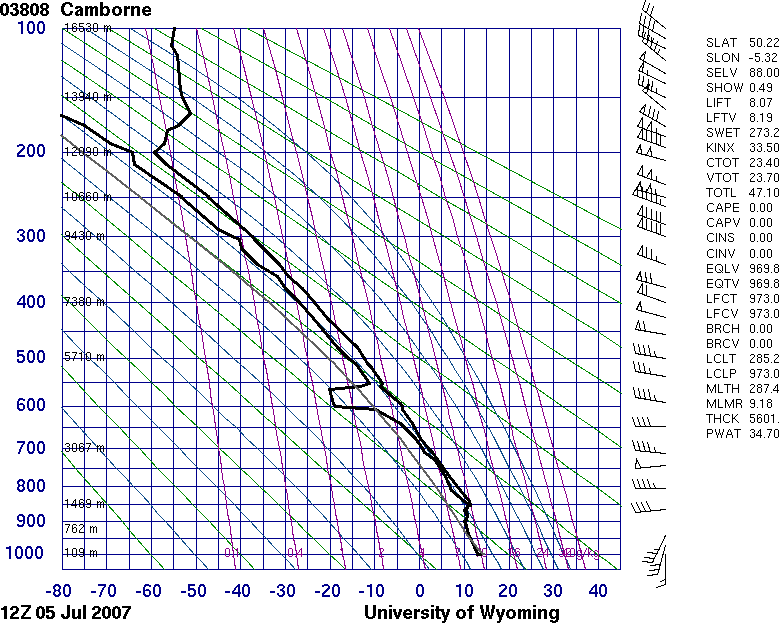
\includegraphics[width=.8\textwidth]{figures/stuve.png}
	\caption{Stuve diagram of 2007-07-05 at 12:00Z \cite{assignment}.}
	\label{fig:Q7}
\end{figure}

%----------------------------------------------------------------------------------------
%	REFERENCES.
%----------------------------------------------------------------------------------------
\newpage				% Start at new page.
\addcontentsline{toc}{section}{References}
\bibliographystyle{ieeetr}
\bibliography{references}



\end{document}
